\documentclass[10pt,a4paper]{article}
\usepackage[UTF8,fontset = windows]{ctex}
\setCJKmainfont[BoldFont=黑体,ItalicFont=楷体]{华文中宋}
\usepackage{amssymb,amsmath,amsfonts,amsthm,mathrsfs,dsfont,graphicx}
\usepackage{ifthen,indentfirst,enumerate,color,titletoc}
\usepackage{tikz}
\usepackage{multicol}
\usepackage{makecell}
\usepackage{longtable}
\usepackage{diagbox}
\usetikzlibrary{arrows,calc,intersections,patterns,decorations.pathreplacing,3d,angles,quotes,positioning}
\usepackage[bf,small,indentafter,pagestyles]{titlesec}
\usepackage[top=1in, bottom=1in,left=0.8in,right=0.8in]{geometry}
\renewcommand{\baselinestretch}{1.65}
\newtheorem{defi}{定义~}
\newtheorem{eg}{例~}
\newtheorem{ex}{~}
\newtheorem{rem}{注~}
\newtheorem{thm}{定理~}
\newtheorem{coro}{推论~}
\newtheorem{axiom}{公理~}
\newtheorem{prop}{性质~}
\newcommand{\blank}[1]{\underline{\hbox to #1pt{}}}
\newcommand{\bracket}[1]{(\hbox to #1pt{})}
\newcommand{\onech}[4]{\par\begin{tabular}{p{.9\textwidth}}
A.~#1\\
B.~#2\\
C.~#3\\
D.~#4
\end{tabular}}
\newcommand{\twoch}[4]{\par\begin{tabular}{p{.46\textwidth}p{.46\textwidth}}
A.~#1& B.~#2\\
C.~#3& D.~#4
\end{tabular}}
\newcommand{\vartwoch}[4]{\par\begin{tabular}{p{.46\textwidth}p{.46\textwidth}}
(1)~#1& (2)~#2\\
(3)~#3& (4)~#4
\end{tabular}}
\newcommand{\fourch}[4]{\par\begin{tabular}{p{.23\textwidth}p{.23\textwidth}p{.23\textwidth}p{.23\textwidth}}
A.~#1 &B.~#2& C.~#3& D.~#4
\end{tabular}}
\newcommand{\varfourch}[4]{\par\begin{tabular}{p{.23\textwidth}p{.23\textwidth}p{.23\textwidth}p{.23\textwidth}}
(1)~#1 &(2)~#2& (3)~#3& (4)~#4
\end{tabular}}
\begin{document}

\begin{enumerate}[1.]

%zmj1
\item 已知集合$A=\{y| y=\sin x , \ x\in \mathbf{R}\}$, 集合$B=\{y| y=\sqrt {x} , \ x\in \mathbf{R}\}$, 则$A\cap B=$\blank{50}.
\item 已知$1+\mathrm{i}$是实系数一元二次方程$x^2+ax+b=0$的根($i$为虚数单位), 则$2a+b=$\blank{50}.
\item 已知关于$x,y$的二元一次方程组的增广矩阵为$\begin{pmatrix}
   2 & 1 & 5  \\ 1 & -2 & 0  \end{pmatrix}$, 则$xy=$\blank{50}.	
\item 已知球的主视图的面积为$\dfrac{\pi}4$, 则该球的体积为\blank{50}.
\item 在平面直角坐标系$xOy$中, 直线$l$的参数方程为$\begin{cases} x=t-1, \\ y=t, \end{cases}$($t$为参数) 圆$O$的参数方程为$\begin{cases} x=\cos \theta,  \\ y=\sin \theta,  \end{cases}$($\theta$为参数) 则直线$l$与圆$O$的位置关系是\blank{50}.
\item 已知实数$x$、$y$满足条件$\begin{cases} x-y\ge 0, \\ y\ge 0, \\ x+y\le 1, \end{cases}$ 则目标函数$z=2x-y$的最大值为\blank{50}.
\item 方程$(\log_3x)^2+\log_93x=2$的解集为\blank{50}.
\item 某校高一、高二、高三共有$200$名学生, 为调查他们的体育锻炼情况, 通过分层抽样获得了20名学生一周的锻炼时间, 数据如下表(单位: 小时):
\begin{center}
\begin{tabular}{|c|c|c|c|c|c|c|c|c|}
\hline
高一 & $6$ & $6.5$ & $7$ & $7.5$ & $8$ & $$ & $$ & $$ \\ \hline
高二 & $6$ & $7$ & $8$ & $9$ & $10$ & $11$ & $12$ & $$ \\ \hline
高三 & $3$ & $4.5$ & $6$ & $7.5$ & $9$ & $10.5$ & $12$ & $13.5$ \\ \hline
\end{tabular}
\end{center}
则根据上述样本数据估计该校学生一周的锻炼时间不小于$7$小时的人数为\blank{50}.
\item 从$m$($m\in \mathbf{N}^*$, $m\ge 4$)个男生、$6$个女生中任选$2$个人当发言人, 假设事件$A$表示选出的$2$个人性别相同, 事件$B$表示选出的$2$个人性别不同. 如果$A$的概率和$B$的概率相等, 则$m=$\blank{50}.
\item 将函数$f(x)=2\sin 2x$的图像向左平移$\dfrac{\pi }6$个单位, 再向下平移$1$个单位, 得到函数的$y=g(x)$图像. 若$y=g(x)$在$[0,b]$($b>0$)上至少含有$2021$个零点, 则$b$的最小值为\blank{50}.
\item 如图, 在$\triangle ABC$中, $\angle BAC=\dfrac{\pi}3$, $D$为$AB$中点, $P$为$CD$上一点, 且满足$\overrightarrow{AP}=t\overrightarrow{AC}+\dfrac 13\overrightarrow{AB}$, 若$\triangle ABC$的面积为$\dfrac{3\sqrt 3}2$, 则$|\overrightarrow{AP}|$的最小值为\blank{50}.
\begin{center}
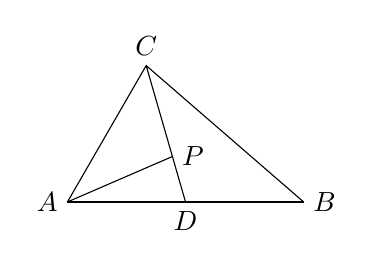
\begin{tikzpicture}[>=latex]
\draw (0,0) node [left] {$A$} coordinate (A) -- (1.5,0) node [below] {$D$} coordinate (D) -- (3,0) node [right] {$B$} coordinate (B);
\draw (60:2) node [above] {$C$} coordinate (C);
\draw ($(C)!{2/3}!(D)$) node [right] {$P$} coordinate (P);
\draw (A) -- (C) -- (B) (A) -- (P) (C) -- (D);
\end{tikzpicture}
\end{center}
\item 已知数列$\{a_n\}$, $\{b_n\}$满足$a_1=b_1=1$, 对任何正整数$n$均有$a_{n+1}=a_n+b_n+\sqrt {a_n^2+b_n^2}$, $b_{n+1}=a_n+b_n-\sqrt {a_n^2+b_n^2}$, 设$c_n=3^n(\dfrac 1{a_n}+\dfrac 1{b_n})$, 则数列$\{c_n\}$的前$2020$项之和为\blank{50}.
\item 已知实数$a\ne 0$, 则``$a<1$''是``$\dfrac 1a>1$''的\blank{50}\bracket{20}
\twoch{充分非必要条件}{必要非充分条件}{充要条件}{既非充分又非必要条件}
\item 如图, 正方体$A_1B_1C_1D_1-ABCD$中, $E$、$F$分别为棱$A_1A$、$BC$上的点, 在平面$ADD_1A_1$内且与平面$DEF$平行的直线\bracket{20}.
\begin{center}
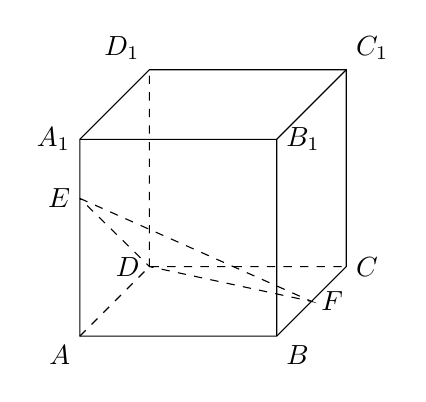
\begin{tikzpicture}[>=latex]
\draw (0,0) node [below left] {$A$} coordinate (A) --++ (2.5,0) node [below right] {$B$} coordinate (B) --++ (45:{2.5/2}) node [right] {$C$} coordinate (C)
--++ (0,2.5) node [above right] {$C_1$} coordinate (C1)
--++ (-2.5,0) node [above left] {$D_1$} coordinate (D1) --++ (225:{2.5/2}) node [left] {$A_1$} coordinate (A1) -- cycle;
\draw (A) ++ (2.5,2.5) node [right] {$B_1$} coordinate (B1) -- (B) (B1) --++ (45:{2.5/2}) (B1) --++ (-2.5,0);
\draw [dashed] (A) --++ (45:{2.5/2}) node [left] {$D$} coordinate (D) --++ (2.5,0) (D) --++ (0,2.5);
\draw ($(B)!0.5!(C)$) node [right] {$F$} coordinate (F);
\draw ($(A)!0.7!(A1)$) node [left] {$E$} coordinate (E);
\draw [dashed] (E) -- (F) -- (D) -- cycle;
\end{tikzpicture}
\end{center}
\fourch{有一条}{有二条}{有无数条}{不存在}
\item 已知函数$f(x)$($x\in D$), 若对任意的$x\in D$, 都存在$t\in D$, 使$f(t)=-f(x)$成立, 称$f(x)$是``拟奇函数''. 下列函数是``拟奇函数''的个数是\bracket{20}.\\
\textcircled{1} $f(x)=x^2$;  \textcircled{2} $f(x)=\ln x$;  \textcircled{3} $f(x)=x+\dfrac 1x$;  \textcircled{4} $f(x)=\cos x$
\fourch{$1$个}{$2$个}{$3$个}{$4$个}
\item 设集合$S=\{1,2,3,\cdots,2020\}$, 设集合$A$是集合$S$的非空子集, $A$中的最大元素和最小元素之差称为集合$A$的直径. 那么集合$S$所有直径为$71$的子集的元素个数之和为\bracket{20}.
\fourch{$71\cdot 1949$}{$2^{70}\cdot 1949$}{$2^{70}\cdot 37\cdot 1949$}{$2^{70}\cdot 72\cdot 1949$}
\item 如图所示的几何体是圆柱的一部分, 它是由边长为$2$的正方形$ABCD$(及其内部)以$AB$边所在直线为旋转轴顺时针旋转$120^{\circ}$得到的.
\begin{center}
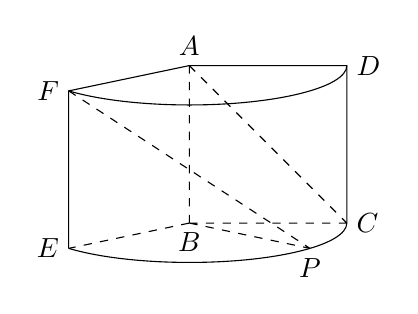
\begin{tikzpicture}[>=latex]
\draw (0,0) node [below] {$B$} coordinate (B);
\draw (2,0) node [right] {$C$} coordinate (C);
\draw (2,2) node [right] {$D$} coordinate (D);
\draw (0,2) node [above] {$A$} coordinate (A);
\draw ({2*cos(-140)},{0.5*sin(-140)}) node [left] {$E$} coordinate (E);
\draw (E) ++ (0,2) node [left] {$F$} coordinate (F);
\draw ({2*cos(-40)},{0.5*sin(-40)}) node [below] {$P$} coordinate (P);
\draw (E) -- (F) -- (A) -- (D) -- (C) arc (0:-140:2 and 0.5);
\draw (D) arc (0:-140:2 and 0.5);
\draw [dashed] (B) -- (A) (B) -- (E) (B) -- (C) (A) -- (C) (F) -- (P) (B) -- (P);
\end{tikzpicture}
\end{center}
(1) 求此几何体的体积;\\
(2) 设$P$是弧$EC$上的一点, 且$BP\perp BE$, 求异面直线$FP$与$CA$所成角的大小. (结果用反三角函数值表示)
\item 已知锐角$\alpha$、$\beta$的顶点与坐标原点重合, 始边与$x$轴正方向重合, 终边与单位圆分别交于$P$、$Q$两点, 若$P$、$Q$两点的横坐标分别为$\dfrac{3\sqrt {10}}{10}$、$\dfrac{2\sqrt 5}5$.\\
(1) 求$\cos (\alpha +\beta)$的大小;\\
(2) 在$\triangle ABC$中, $a,b,c$为三个内角$A,B,C$对应的边长, 若已知角$C=\alpha +\beta$, $\tan A=\dfrac 34$, 且$a^2=\lambda bc+c^2$, 求$\lambda$的值.
\item 疫情后, 为了支持企业复工复产, 某地政府决定向当地企业发放补助款, 其中对纳税额在$3$万元至$6$万元(包括$3$万元和$6$万元)的小微企业做统一方案. 方案要求同时具备下列两个条件: \textcircled{1} 补助款$f(x)$(万元)随企业原纳税额$x$(万元)的增加而增加; \textcircled{2} 补助款不低于原纳税额$x$(万元)的$50\%$. 经测算政府决定采用函数模型$f(x)=\dfrac x4-\dfrac bx+4$(其中$b$为参数)作为补助款发放方案.\\
(1) 判断使用参数$b=12$是否满足条件, 并说明理由;\\
(2) 求同时满足条件\textcircled{1}、\textcircled{2}的参数$b$的取值范围.
\item 在平面直角坐标系$xOy$中, $F_1$, $F_2$分别是椭圆$\Gamma :\dfrac{x^2}{a^2}+y^2=1$($a>0$)的左、右焦点, 直线$l$与椭圆交于不同的两点$A$, $B$, 且$|AF_1|+|AF_2|=2\sqrt 2$.\\
(1) 求椭圆$\Gamma$的方程;\\
(2) 已知直线$l$经过椭圆的右焦点$F_2$, $P,Q$是椭圆上两点, 四边形$ABPQ$是菱形, 求直线$l$的方程;\\
(3) 已知直线$l$不经过椭圆的右焦点$F_2$, 直线$AF_2$, $l$, $BF_2$的斜率依次成等差数列, 求直线$l$在$y$轴上截距的取值范围.
\item 若数列$\{a_n\}$对任意连续三项$a_i,a_{i+1},a_{i+2}$, 均有$(a_i-a_{i+2})(a_{i+2}-a_{i+1})>0$, 则称该数列为``跳跃数列''.\\
(1) 判断下列两个数列是否是跳跃数列:\\
\textcircled{1} 等差数列: $1,2,3,4,5,\cdots$; \textcircled{2} 等比数列: $1,-\dfrac 12,\dfrac 14,-\dfrac 18,\dfrac 1{16},\cdots$;\\
(2) 若数列$\{a_n\}$满足对任何正整数$n$, 均有$a_{n+1}=a_1^{a_n}$($a_1>0$). 证明: 数列$\{a_n\}$是跳跃数列的充分必要条件是$0<a_1<1$;\\
(3) 跳跃数列$\{a_n\}$满足对任意正整数$n$均有$a_{n+1}=\dfrac{19-a_n^2}5$, 求首项$a_1$的取值范围.

%zmj2
\item 已知集合$A=\{y|y=10^x, \ x\in \mathbf{R}\}$, $B=\{y|y=x^2, \ 1\le x\le 2\}$, 则$A\cap B=$\blank{50}.
\item $\displaystyle\lim_{n\to\infty}\dfrac{3^n-1}{3^n+1}=$\blank{50}.
\item 若关于$x, y$的方程组$\begin{cases}x+y=m, \\ x+ny=1\end{cases}$有无穷多组解, 则$m+n$的值为\blank{50}.
\item 若$-1+2\mathrm{i}$($\mathrm{i}$为虚数单位)是方程$x^2+bx+c=0$($b$、$c\in \mathbf{R}$)的一个根, 则$c-b=$\blank{50}.
\item 已知$P$为抛物线$C:y^2=2px(p>0)$上一点, 点$P$到抛物线$C$的焦点的距离为$7$, 到$y$轴的距离为$5$, 则$p=$\blank{50}.
\item 设复数$z=\begin{vmatrix}\cos \alpha & \mathrm{i} \\ \sin \alpha  & \sqrt 2+\mathrm{i} \end{vmatrix}$($\mathrm{i}$为虚数单位), 若$|z|=\sqrt 2$, 则$\tan 2\alpha =$\blank{50}.
\item 若$(ax^2+\dfrac 1{\sqrt x})^{5}$的展开式中的常数项为$-\dfrac 5{2}$, 则实数$a$的值为\blank{50}.
\item 设函数$f(x)$的定义域为$D$. 若对于$D$内的任意$x_1$, $x_2$($x_1\ne x_2$), 都有$(x_2-x_1)[f(x_2)-f(x_1)]>0$, 则称函数$f(x)$为``Z函数''.有下列函数: \textcircled{1} $f(x)=1$; \textcircled{2} $f(x)=-2x+1$; \textcircled{3} $f(x)=x^3$; \textcircled{4} $f(x)=\lg x$. 其中``Z函数''的序号是\blank{50}(写出所有的正确序号).
\item 已知直三棱柱的各棱长都相等, 体积等于$18$($\text{cm}^3$). 若该三棱柱的所有顶点都在球$O$的表面上, 则球$O$的体积等于\blank{50}($\text{cm}^3$).
\item 已知$F_1,F_2$是椭圆$C:\dfrac{x^2}{a^2}+\dfrac{y^2}3=1$($a>\sqrt 3$)的左、右焦点, 过原点$O$且倾斜角为$60^\circ$的直线与椭圆$C$的一个交点为$M$. 若$|\overrightarrow{MF_1}+\overrightarrow{MF_2}|=|\overrightarrow{MF_1}-\overrightarrow{MF_2}|$, 则椭圆$C$的长轴长为\blank{50}.
\item 已知无穷等比数列$a_1,a_2,a_3,\cdots$各项的和为$\dfrac 92$, 且$a_2=-2$, 若$|S_n-\dfrac 92|<10^{-4}$, 则$n$的最小值为\blank{50}.
\item 若同一平面上不共线的四个点$P,Q,R,S$满足: $mn\overrightarrow{RP}=n(1-3m)\overrightarrow{QP}+m(n-1)\overrightarrow{SP}$($m>0$、$n>0$), 则当$\triangle PRS$的面积是$\triangle PQR$的面积的$\dfrac 13$倍时, $\dfrac1{m+n}$的最大值为\blank{50}.
\item 设$x\in \mathbf{R}$, 则``$x>3$''是``$x^2>9$'' 的\bracket{20}.
\twoch{充分非必要条件}{必要非充分条件}{充要条件}{既非充分条件又非必要条件}
\item 某班有学生$40$人, 将这$40$人编上$1$到$40$的号码, 用系统抽样的方法抽取一个容量为$4$的样本. 已知编号为$3$、$23$、$33$的学生在样本中, 则另一学生在样本中的编号为\bracket{20}.
\fourch{$12$}{$13$}{$14$}{$15$}
\item 已知函数$f(x)=\sin(\omega x+\dfrac{\pi}6)+\dfrac 12$($\omega >0)$在区间$(0,\dfrac{\pi}2)$上有且仅有两个零点, 则实数$\omega$的取值范围为\bracket{20}.
\fourch{$(2, \dfrac{14}{3}]$}{$[2,\dfrac{14}{3})$}{$[\dfrac{10}{3}, 4)$}{$(\dfrac{10}{3}, 6]$}
\item 如果数列$u_1, u_2, \cdots, u_{10}$同时满足以下四个条件: \textcircled{1} $u_i\in \mathbf{Z}$($i=1, 2, \cdots, 10$); \textcircled{2} 点$(u_5, 2^{u_2+u_8})$在函数$y=4^x$的图像上; \textcircled{3} 向量$\overrightarrow a=(1, u_1)$与$\overrightarrow b=(3, u_{10})$互相平行;
\textcircled{4} $u_{i+1}-u_i$与$\dfrac2 {u_{i+1}-u_i}$的等差中项为$\dfrac 32$($i=1, 2, \cdots, 9$). 那么, 这样的数列$u_1, u_2, \cdots, u_{10}$的个数为\bracket{20}.
\fourch{$78$}{$80$}{$82$}{$90$}
\item 在三棱锥$P-ABC$中, $PA=PB=PC=AC=2\sqrt 2$, $BA=BC=2$, $O$是线段$AC$的中点, $M$是线段$BC$的中点.
\begin{center}
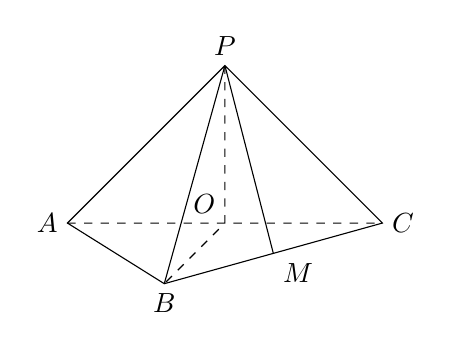
\begin{tikzpicture}[>=latex]
\draw (0,0,0) node [above left] {$O$} coordinate (O);
\draw (2,0,0) node [right] {$C$} coordinate (C);
\draw (-2,0,0) node [left] {$A$} coordinate (A);
\draw (0,0,2) node [below] {$B$} coordinate (B);
\draw (0,2,0) node [above] {$P$} coordinate (P);
\draw ($(B)!0.5!(C)$) node [below right] {$M$} coordinate (M);
\draw (A) -- (P) -- (C) -- (B) -- cycle (P) -- (B) (P) -- (M);
\draw [dashed] (A) -- (C) (P) -- (O) -- (B);
\end{tikzpicture}
\end{center}
(1) 求证: $PO\perp$平面$ABC$;\\
(2) 求直线$PM$与平面$PBO$所成的角的大小.
\item 将关于$x$的函数$y=\dfrac{m(x+2)^2}x$($m\in \mathbf{R}$)的图像向右平移$2$个单位后得到的函数图像记为$C$, 并设$C$所对应的函数为$f(x)$.\\
(1) 当$m>0$时, 试直接写出函数$f(x)$的单调递减区间;\\
(2) 设$f(4)=8$, 若函数$g(x)=x^2-2ax+5$($a>1$)对于任意$t_1\in [0, 1]$, 总存在$t_2\in [0, 1]$, 使得$g(t_2)=f (t_1)$成立, 求$a$的取值范围.
\item 某工厂制作如图所示的一种标识, 在半径为$R$的圆内作一个关于圆心对称的 ``H''型图形, ``H''型图形由两竖一横三个等宽的矩形组成, 两个竖直的矩形全等且它们的长边是横向矩形长边的$\dfrac{3}{2}$倍, 设$O$为圆心, $\angle AOB=2\alpha$, 记``H''型图形的面积为$S$.
\begin{center}
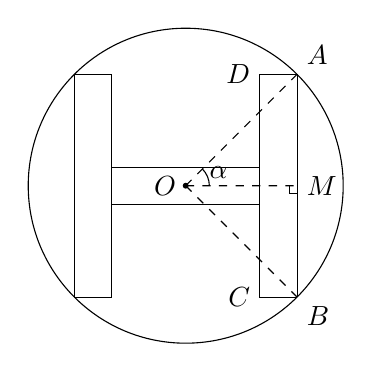
\begin{tikzpicture}[>=latex]
\draw (0,0) circle (2) node [left] {$O$} coordinate (O);
\filldraw (0,0) circle (0.03);
\draw (45:2) node [above right] {$A$} coordinate (A);
\draw (-45:2) node [below right] {$B$} coordinate (B);
\draw ($(A)!0.5!(B)$) node [right] {$M$} coordinate (M);
\draw [dashed] (O) -- (M) (O) -- (A) (O) -- (B);
\draw (O) pic ["$\alpha$",draw,angle eccentricity = 1.5, scale = 0.6] {angle = M--O--A};
\draw (A) -- (B);
\draw (A) ++ ({-sqrt(2)/3},0) node [left] {$D$} coordinate (D);
\draw (B) ++ ({-sqrt(2)/3},0) node [left] {$C$} coordinate (C);
\draw (A) -- (D) -- (C) -- (B);
\draw (M) pic [draw,scale = 0.2] {right angle = O--M--B};
\draw ({sqrt(2)*2/3},{sqrt(2)/6}) -- ({-sqrt(2)*2/3},{sqrt(2)/6});
\draw ({sqrt(2)*2/3},{-sqrt(2)/6}) -- ({-sqrt(2)*2/3},{-sqrt(2)/6});
\draw (135:2) --++ ({sqrt(2)/3},0) --++ (0,{-2*sqrt(2)}) --++ ({-sqrt(2)/3},0) --cycle;
\end{tikzpicture}
\end{center}
(1) 将$AB,AD$用$R,\alpha$表示, 并将$S$表示成$\alpha$的函数;\\
(2) 为了突出``H''型图形, 设计时应使$S$尽可能大, 则当$\alpha$为何值时, $S$最大? 并求出$S$的最大值.
\item 已知椭圆$C$的方程为$\dfrac{x^2}2+y^2=1$.、、
(1) 设$M(x_M,y_M)$是椭圆$C$上的点, 证明: 直线$\dfrac{x_Mx}2+y_My=1$与椭圆$C$有且只有一个公共点;\\
(2) 过点$N(1,\sqrt 2)$作两条与椭圆只有一个公共点的直线, 公共点分别记为$A$、$B$, 点$N$在直线$AB$上的射影为点$Q$, 求点$Q$的坐标;\\
(3) 互相垂直的两条直线$l_1$与$l_2$相交于点$P$, 且$l_1$、$l_2$都与椭圆$C$只有一个公共点, 求证点$P$落在$x^2+y^2=3$上.
\item 若数列$\{a_n\}$满足``对任意正整数$i$, $j$, $i\ne j$, 都存在正整数$k$, 使得$a_k=a_i\cdot a_j$'', 则称数列$\{a_n\}$具有``性质$P$''.\\
(1) 判断各项均等于$a$的常数列是否具有``性质$P$'', 并说明理由;\\
(2) 若公比为$2$的无穷等比数列$\{a_n\}$具有``性质$P$'', 求首项$a_1$的值;\\
(3) 若首项$a_1=2$的无穷等差数列$\{a_n\}$具有``性质$P$'', 求公差$d$的值.


\end{enumerate}


\iffalse



\item 设集合$A=\{1,2,3,4\}$, 集合$B=\{1,3,5,7\}$, 则$A\cap B=$\blank{50}.
\item 行列式$\begin{vmatrix}1  2  0 \\2  3  5 \\5  8  0\end{vmatrix}$的值为\blank{50}.
\item 函数$y=\dfrac{\cos ^2x+1}2$的最小正周期为\blank{50}.
\item 设$\mathrm{\mathrm{i}}$是虚数单位, 复数$z$满足$(1+2\mathrm{i})z=|4+3\mathrm{i}|$, 则$z=$\blank{50}.
\item 若$\{a_n\}$是无穷等比数列, 首项$a_2=1$, 公比$q=\dfrac 13$, 则$\{a_n\}$各项的和$S=$\blank{50}.
\item 在$4$名男生, $4$名女生中随机选出$3$名学生参加某次活动, 则选出的学生中至多$1$名女生的概率为\blank{50}(结果用最简分数表示).
\item 实数$x,y$满足约束条件$\begin{cases}x+2y\le 4, \\2x+y\le 3, \\x\ge 0, \\y\ge 0\end{cases}$, 目标函数$z=x+y$的最大值为\blank{50}.
\item 已知曲线$C_1$的参数方程为$\begin{array}*35l
   x=\sqrt 3t-1  \\y=t+\sqrt 3  \end{array}$($t$是参数), 曲线$C_2$的参数方程为$\begin{array}*35l
   x=-2+\sqrt 5\cos \theta   \\y=\sqrt 5\sin \theta   \end{array}$($\theta$是参数), 则$C_1$和$C_2$的两个交点之间的距离为\blank{50}.
\item 数列$\{a_n\}$满足$a_1=1$, 且$a_n+a_{n+1}=3n+2$对任意$n\in \mathbf{N}^*$均成立, 则$a_{2022}=$\blank{50}.
\item 设$n\in \mathbf{N}^*$, 若$(2+\sqrt x)^n$的二项展开式中, 有理项的系数之和为$365$, 则$n=$\blank{50}.
\item 设$\veca$、$\vecb$、$\vecc$是同一平面上的三个两两不同的单位向量. 若$(\veca\cdot \vecb):(\vecb\cdot \vecc):(\vecc\cdot \veca)$
 $=1:1:3$, 则$\veca\cdot\vecb$的值为\blank{50}.
\item 设$n\in \mathbf{N}^*$, 圆$C_n$: $x^2+y^2=R_n^2\ (R_n>0)$与$y$轴正半轴的交点为$M$, 与曲线$y=\sqrt x$的交点为$N(x_n,y_n)$, 直线$MN$与$x$轴的交点为$A(a_n,0)$.若数列$\{x_n\}$满足: $x_{n+1}=4x_n+3,x_1=3$.
则常数$p$=\blank{50}使数列$\{a_{n+1}-p\cdot a_n\}$成等比数列.
二、选择题
\item 不等式$\dfrac{x-1}{x-2}\le 0$的解集为\blank{50}\bracket{20}.
\fourch{$[1,2]$}{$[1,2)$}{$(-\infty,1]\cup [2,+\infty)$}{$(-\infty,1)\cup (2,+\infty)$}
\item 设$z$是复数, 则``$z$是虚数''是``$z^3$是虚数''的\blank{50}		 \bracket{20}.
\fourch{充分非必要条件}{必要非充分条件}{充要条件}{既不充分又不必要条件}
\item 设$F_1,F_2$是椭圆$\dfrac{x^2}9+\dfrac{y^2}4=1$的两焦点, $A$与$B$分别是该椭圆的右顶点与上顶点. $P$是该椭圆上的一个动点, $O$是坐标原点. 记$s=\overrightarrow{F_1P}\cdot \overrightarrow{F_2P}-2\overrightarrow{OP}^2$. 在动点$P$在第一象限内从$A$沿椭圆向左上方运动到$B$的过程中, $s$的大小的变化情况为\blank{50}									 \bracket{20}.
\fourch{逐渐变大}{逐渐变小}{先变大后变小}{先变小后变大}
\item 设$\{a_n\}$是$2022$项的实数数列, $\{a_n\}$中的每一项都不为零. $\{a_n\}$中任意连续$11$项$a_n,a_{n+1},\cdots ,a_{n+10}$的乘积是定值($n=1,2,3,\cdots ,2012$). 命题
\textcircled{1}  不存在满足条件的数列, 使得其中恰有$365$个$1$;
\textcircled{2}  存在满足条件的数列, 使得其中恰有$550$个$1$;
的真假情况为\blank{50}	\bracket{20}.
\fourch{\textcircled{1} 和\textcircled{2} 都是真命题}{\textcircled{1} 是真命题, \textcircled{2} 是假命题}{\textcircled{2} 是真命题, \textcircled{1} 是假命题}{\textcircled{1} 和\textcircled{2} 都是假命题}
三、解答题
\item 如图, 线段$OA$和$OB$是以$P$为顶点的圆锥的底面上的两条相互垂直的半径. 点$M$是母线$BP$的中点. 已知$OA=OM=2$.
(1) 求该圆锥的体积;
(2) 求异面直线$OM$与$AP$所成的角的大小.
\item 已知三角形$ABC$中, 三个内角$ABC$的对应边分别为$a$、$b$、$c$, 且$a=5$, $b=7$.
(1) 若$B=\dfrac{\pi }3$, 求$c$;
(2) 设点$M$是边$AB$的中点, 若$CM=3$, 求三角形$ABC$的面积.
\item 某地出现了虫害. 农业科学家引入了``虫害指数''数列$\{I_n\}$, $\{I_n\}$表示第$n$周的虫害的严重程度, 虫害指数越大, 严重程度越高. 为了治理虫害, 需要环境整治、杀灭害虫, 然而由于人力资源有限, 每周只能采取以下两个策略之一:
策略A: 环境整治, ``虫害指数''数列满足$I_{n+1}=1.02I_n-0.20$;
策略B: 杀灭害虫, ``虫害指数''数列满足$I_{n+1}=1.08I_n-0.46$;
当某周``虫害指数''小于$1$时, 危机就在这周解除 .
(1) 设第一周的虫害指数$I_1\in [1,8]$, 用哪一个策略将使第二周的虫害的严重程度更小?
(2) 设第一周的虫害指数$I_1=3$, 如果每周都采用最优的策略, 虫害的危机最快在第几周解除?
\item 已知双曲线$H:x^2-\dfrac{y^2}{b^2}=1(b>0)$, 经过点$D(2,0)$的直线$l$与该双曲线交于$M$、$N$两点.
(1) 若$l$与$x$轴垂直, 且$|MN|=6$, 求$b$的值;
(2) 若$b=\sqrt 2$, 且$M$、$N$的横坐标之和为$-4$, 证明: $\angle MON=90^\circ$;
(3) 设直线$l$与$y$轴交于点$E$, $\overrightarrow{EM}=\lambda \cdot \overrightarrow{MD}$, $\overrightarrow{EN}=\mu \cdot \overrightarrow{ND}$, 求证: $\lambda +\mu$为定值.
\item $f(x)=2^{x+m}+m x+1$, 其中$m$是实常数.
(1) 若$f(\dfrac 1m)>18$, 求$m$的取值范围;
(2) 若$m>0$, 求证: 函数$f(x)$的零点有且仅有一个;
(3) 若$m>0$, 设函数$y=f(x)$的反函数为$y=f^{-1}(x)$, 若$a_1,a_2,a_3,a_4$是公差$d>0$的等差数列且均在函数$f(x)$的值域中, 求证: $f^{-1}(a_1)+f^{-1}(a_4)<f^{-1}(a_2)+f^{-1}(a_3)$.


2022届高三下数学周末卷4   班级学号\blank{50}姓名\blank{50}
一、填空题
\item 已知集合$U=\{-1,0,1,2,3\}$, $A=\{-1,0,2\}$, 则$C_UA=$\blank{50}.
\item 已知一个关于$x$、$y$的二元一次方程组的增广矩阵是$\begin{pmatrix}
   1  -1  1  \\0  1  2  \end{pmatrix}$, 则$x+y=$\blank{50}.
\item $\mathrm{i}$是虚数单位, 若复数$(1-2\mathrm{i})(a+\mathrm{i})$是纯虚数, 则实数$a$的值为\blank{50}.
\item 已知二项式$(x^2+\dfrac ax)^6$的展开式中含$x^3$项的系数是160, 则实数$a$的值是\blank{50}.
\item 直线$l$的参数方程为$\begin{cases} x=1+t \\ y=-1+2t \end{cases}$($t$为参数), 则$l$的一个法向量为\blank{50}.
\item 已知某圆锥的正视图是边长为2的等边三角形, 则该圆锥的体积等于\blank{50}.
\item 已知椭圆$\dfrac{x^2}{a^2}+y^2=1$($a>0$)的左右焦点分别为$F_1$、$F_2$, 抛物线$y^2=2x$的焦点为$F$, 若$\overrightarrow{F_1F}=3\overrightarrow{FF_2}$, 则$a=$\blank{50}.
\item 甲、乙、丙、丁4名同学参加志愿者服务, 分别到三个路口疏导交通, 每个路口有1名或2名志愿者, 则甲、乙两人在同一路口的概率为\blank{50}.
\item 将函数$f(x)=\sin x$的图像向右平移$\varphi (\varphi >0)$个单位后得到函数$y=g(x)$的图像. 若对满足$|f(x_1)-g(x_2)|=2$的任意$x_1$、$x_2$, $|x_1-x_2|$的最小值是$\dfrac{\pi }3$, 则$\varphi$的最小值是\blank{50}.
\item 如图, 已知AB是边长为1的正六边形的一条边,
P在正六边形内(含边界), 则$\overrightarrow{AP}\cdot \overrightarrow{BP}$的取值范围是\blank{50}.
\item 已知曲线C: $y=\dfrac 2x\begin{matrix}
     \end{matrix}(1\le x\le 2)$, 若对于曲线C上的任意一点$P(x,y)$, 都有$(x+y+c_1)(x+y+c_2)\le 0$, 则$|c_1-c_2|$的最小值为\blank{50}.
\item 在数列 中, $a_1=3$, , 记 为数列 的前 项和, 则 =\blank{50}.
二、选择题
\item 设$\overrightarrowa$、$\overrightarrowb$分别是两条异面直线$l_1$、$l_2$的方向向量, 向量$\overrightarrowa$、$\overrightarrowb$夹角的取值范围为$A$, $l_1$、
$l_2$所成角的取值范围为$B$, 则``$\alpha \in A$''是``$\alpha \in B$''的\bracket{20}.
\fourch{充要条件}{充分不必要条件}{必要不充分条件}{ 既不充分也不必要条件}
\item 若等比数列$\{a_n\}$的公比为$q$, 则关于$x$、$y$的二元一次方程组$\begin{cases} a_1x+a_5y=2 \\ a_2x+a_6y=1 \end{cases}$的解的情况下列说法正确的是\bracket{20}.
\fourch{对任意$q\in \mathbf{R}$($q\ne 0$), 方程组有唯一解}{对任意$q\in \mathbf{R}$($q\ne 0$), 方程组都无解}{当且仅当$q=\dfrac 12$时, 方程组有无穷多解}{当且仅当$q=\dfrac 12$时, 方程组无解}
\item 已知实数 、 满足 , 有结论:
\textcircled{1}  当 时, 存在最大值;
\textcircled{2}  当$a<0,b<0$时, 存在最小值.  正确的判断是\bracket{20}.
\fourch{ \textcircled{1} 成立, \textcircled{2} 成立}{ \textcircled{1} 不成立, \textcircled{2} 不成立}{ \textcircled{1} 成立, \textcircled{2} 不成立}{ \textcircled{1} 不成立, \textcircled{2} 成立}
\item 已知函数$f(x)=\dfrac 1x+|2x-a|$. 若存在相异的实数$x_1,x_2\in (-\infty ,0)$, 使得$\begin{cases}  \\ : 13164776105~ \\ www.jyeoo.com \end{cases}$成立, 则实数$\begin{cases}  \\ : 13164776105~ \\ www.jyeoo.com \end{cases}$的取值范围为\bracket{20}.
\fourch{}{}{}{}
三、解答题
\item 已知在直三棱柱$ABC-A_1B_1C_1$中, $\angle BAC=90^\circ \ AB=BB_1=1$, 直线$B_1C$与平面ABC成$30^\circ$的角.
(2)	求三棱锥$C_1-AB_1C$的体积;
(2)求二面角$B-B_1C-A$的余弦值.
\item 已知复数$z$满足$|z|=\sqrt 2$, $z^2$的虚部为$2$.
(1)求复数$z$;
(2)设复数$zz^2z-z^2$在复平面上对应的点分别为$ABC$, 求: $(\overr\mathrm{i}ghtarrow{OA}+\overr\mathrm{i}ghtarrow{OB})\cdot \overr\mathrm{i}ghtarrow{OC}$的值.
\item 某公园内有一块以O为圆心半径为20米的圆形区域. 为丰富市民的业余文化生活, 现提出如下设计方案: 如图, 在圆形区域内搭建露天舞台, 舞台为扇形OAB区域, 其中两个端点A, B分别在圆周上; 观众席为等腰梯形ABQP内且在圆O外的区域, 其中$AP=AB=BQ$, $\angle PAB=\angle QBA=\dfrac{2\pi }3$, 且$AB\ PQ$在点O的同侧. 为保证视听效果, 要求观众席内每一个观众到舞台中心O处的距离都不超过60米(即要求$PO\le 60$). 设$\angle OAB=\alpha ,\ \alpha \in (0,\ \dfrac{\pi }3)$.
(1)当$\alpha =\dfrac{\pi }6$时, 求舞台表演区域的面积;
(2)对于任意$\alpha$, 上述设计方案是否均能符合要求?
\item 双曲线$C:x^2-\dfrac{y^2}{b^2}=1\ (b>0)$的左顶点为A, 右焦点为F, 点B是双曲线C上一点.
(1)当$b=2$时, 求双曲线两条渐近线的夹角;
(2)若直线BF的倾斜角为$\dfrac{\pi }4$, 与双曲线C的另一交点为D, 且$|BD|=8$, 求$b$的值;
(3)若$\overrightarrow{AF}\cdot \overrightarrow{BF}=0$, 且$|\overrightarrow{AF}|=|\overrightarrow{BF}|$, 点E是双曲线C上位于第一象限的动点,
求证: $\angle EFA=2\angle EAF$.
\item 设数列$\{a_n\}$的前$n$项和为$S_n$, 若$\dfrac 12\le \dfrac{a_{n+1}}{a_n}\le 2$($n\in \mathbf{N}^*$), 则称$\{a_n\}$是``紧密数列''.
(1)已知数列$\{a_n\}$是``紧密数列'', 其前5项依次为$1,\dfrac 32,\dfrac 94,x,\dfrac{81}{16}$, 求$x$的取值范围;
(2)若数列$\{a_n\}$的前$n$项和为$S_n=\dfrac 14(n^2+3n)$($n\in \mathbf{N}^*$), 判断$\{a_n\}$是否是``紧密数列'',
并说明理由;
(3)设$\{a_n\}$是公比为$q$的等比数列, 若$\{a_n\}$与$\{S_n\}$都是``紧密数列'', 求$q$的取值范围.

2022届高三(下)周末卷5
姓名:\blank{50}班级学号:\blank{50}
一、填空题.
\item 行列式
\item 的值为\blank{50}.
\item 设集合$A=\{x|y=\sqrt {x-1}x\in \mathbf{R}\}$, $B=\{y|y=\sqrt {1-x^2}x\in \mathbf{R}\}$, 则$A\cap B=$\blank{50}.
\item 若函数$f(x)=1+\dfrac 1x(x>0)$的反函数为$f^{-1}(x)$, 则不等式$f^{-1}(x)>2$的解集为\blank{50}.
\item 已知常数$a>0$, 双曲线$4x^2-y^2=1$的一条渐近线与直线$ax+y+1=0$垂直, 则	$a=$\blank{50}.
\item 以抛物线$y^2=4x$的焦点为圆心, 且与该抛物线的准线相切的圆的标准方程	为\blank{50}.
\item 若$\log__ab=-2$, 则$a^2+b$的取值范围为\blank{50}.
\item 在一个水平放置的底面半径为$\sqrt 3$的的圆柱形量杯中装有适量的水, 现放入一个半径为	$R$的实心铁球, 球完全浸没入水中且无水溢出. 若水面上升高度也为$R$, 则	$R=$\blank{50}.
\item 若$\alpha \in (\dfrac{\pi }4,\dfrac{\pi }2)$, $\sin 2\alpha =\dfrac 1{16}$, 则$\cos \alpha -\sin \alpha =$\blank{50}.
\item 在平面直角坐标系$xOy$中, 将点$A(2,1)$绕原点$O$逆时针旋转$\dfrac{\pi }4$到点$B$. 设直线$OB$的倾	斜角为$\alpha$, 则$\cos \alpha =$\blank{50}.
\item 已知数列$\{a_n\}$满足$a_{n+1}+a_n=4n+2$. 若$\{a_n\}$单调递增, 则$a_1$的取值范围为\blank{50}.
\item 已知复数$z_1,z_2$满足$|z_1|\le 1$, $-1\le \mathbf Rez_2\le 1$, $-1\le \mathbf Imz_2\le 1$. 设$z=z_1+z_2$, 则$z$在复平面	上对应的点组成的图形的面积为\blank{50}.
\item 已知椭圆$\Gamma \dfrac{x^2}2+y^2=1$的左、右焦点分别为$F_1,F_2$, 点$A$为椭圆$\Gamma$的上顶点, 坐标平面内	的动点$P$满足$|AP|^2=2\overrightarrow{PF_1}\cdot \overrightarrow{PF_2}$, 则$|\overrightarrow{PF_1}+2\overrightarrow{PF_2}|$的最大值为\blank{50}.
二、选择题.
\item 若$\cos \alpha >0$, $\sin 2\alpha <0$, 则角$\alpha$的终边所在象限是\bracket{20}.
	\fourch{第一象限}{第二象限}{第三象限}{第四象限}
\item 过抛物线$y^2=8x$的焦点作直线与抛物线相交于两点, 且这两点的横坐标之和$9$, 则满足	条件的直线\bracket{20}.
	\fourch{有$1$条}{有$2$条}{有无穷多条}{不存在}
 
\item 在$(\sqrt x+\dfrac 2{x^2})^n(n\in \mathbf{N}^*)$的展开式中, 设含有$(\sqrt x)^{n-r}(\dfrac 2{x^2})^r$的项为第$r+1(0\le r\le nn\in \mathbf{N})$	项. 若第$3$项与第$5$项的系数之比为$3:56$, 则展开式中的常数项为\bracket{20}.
	\fourch{$180$}{$160$}{$120$}{$100$}
\item 已知等差数列$\{a_n\}$与等比数列$\{b_n\}$都不是常数列. 设集合$S=\{k|a_k=b_kk\in \mathbf{N}^*\}$, 则$S$	元素个数的最大值为\bracket{20}.
	\fourch{$2$}{$3$}{$4$}{$5$}
三、解答题.
\item 如图, 在$\mathbf{R}t\triangle ABC$中, $AB\perp AC$. $PA\perp$平面$ABC$, $D$为$AC$的中点. 过点$D$作$DE\perp$平面$ABC$, $DE<AP$, 连结$BP,BE$.
(1)作出平面$PBE$与平面$ABC$的交线(保留作图痕迹);
(2)若$PA=AC=2$, $DE=1$, 四棱锥$B-ADEP$的体积为$\dfrac{\sqrt 3}3$, 求平面$PBE$与平面$ABC$所成锐二面角的大小.
\item 设函数$f(x)=2\sin (x+\dfrac{\pi }3)\cos x$.
(1)求$f(x)$在$[0,\dfrac{\pi }2]$上的值域;
	(2)记$\triangle ABC$三个内角$A,B,C$的对边分别为$a,b,c$. 若$A$为锐角, $f(A)=\dfrac{\sqrt 3}2$, $b=2$, $c=3$, 求$\cos (A-B)$的值.
\item 某企业参加A项目生产的工人为$1000$人, 平均每人每年创造利润$10$万元. 根据现实的需要, 从A项目中调出$x$人参与B项目的售后服务工作, 每人每年可以创造利润$10(a-\dfrac{3x}{500})$万元(其中常数$a>0$), A项目余下的工人每人每年创造利润需要提高$0.2x%$.
(1)若要保证A项目余下的工人创造的年总利润不低于原来$1000$名工人创造的年总利润, 则最多调出多少人参加B项目从事售后服务工作?
	(2)当从A项目调出的人数不超过总人数的$40%$时, 总能使得A项目中留岗工人创造的年总利润不低于调出的工人所创造的年总利润, 求$a$的取值范围.
 
\item 已知常数$k>0$, 在平面直角坐标系$xOy$中, $A,B$两点分别在第一象限、第四象限, 直线$OA,OB$的一个方向向量分别为$\overrightarrow{d_1}=(1,k)$, $\overrightarrow{d_2}=(1,-k)$, 动点$P$在$\angle AOB$内, 过点$P$分别作$PM\perp OA$于$M$, $PN\perp OB$于$N$.
(1)若$k=1$, $P(\dfrac 32,\dfrac 12)$, 求$|OM|$的值;
(2)若$P(2,1)$, $\triangle OMP$的面积为$\dfrac 65$, 求$k$的值;
(3)设线段$MN$的中点为$T$. 当$\triangle MON$的面积为$\dfrac 1k$时, 求证: $|OT|\ge \dfrac 1k$.
\item 若无穷数列$\{a_n\}$满足: 存在互异的$p,q\in \mathbf{N}^*$使得$a_p=a_q$, 且对任意$n\in \mathbf{N}^*$, 当$n\ne p$且$n\ne q$时, 恒有$a_n>a_p$, 则称$\{a_n\}$具有性质$P$.
	(1)已知常数$k\in \mathbf{N}^*$, 无穷数列$\{a_n\}$的通项公式为$a_n=n+\dfrac kn$. 若$\{a_n\}$具有性质$P$, 求$k$的值;
	(2)已知常数$\lambda \in \mathbf{R}$, 无穷数列$\{a_n\}$的通项公式为$a_n=\begin{cases} -2n+111\le n\le 5 \\ 2^{n-5}+\lambda n\ge 6. \end{cases}$若$\{a_n\}$具有性质$P$, 求$\lambda$的值以及$\{a_n\}$的前$n$项和$S_n$;
	(3)已知常数$t\in \mathbf{Z}$, 无穷数列$\{a_n\}$的通项公式为$a_n=(tn+3)(\dfrac 9{10})^n$. 问: 是否存在$t$, 使得$\{a_n\}$具有性质$P$? 若存在, 求出所有$t$的值; 若不存在, 说明理由.
.


2022届高三下数学周末卷6\blank{50}班级学号\blank{50}姓名\blank{50}
一. 填空题
\item 的展开式中 项的系数是\blank{50}.
\item 设变量x, y满足约束条件 则 的最大值为\blank{50}.
\item 已知奇函数 的周期为2, 且当 时,\blank{50}. 则 的值为\blank{50}.
\item 一个几何体的三视图如图所示, 则这个几何体的表面积为\blank{50}.
\item 投掷两颗六个面上分别刻有1到6的点数的均匀的骰子, 得到其向上的点数分别为 和 , 则复数  为虚数的概率为\blank{50}.
\item 某茶农打算在自己的茶园建造一个容积为500立方米的长方体无盖蓄水池, 要求池底面的长和宽之和为20米. 若每平方米的池底面造价是池侧壁的两倍, 则为了使蓄水池的造价最低, 蓄水池的高应该为\blank{50}米.
\item 如图, 在直角梯形ABCD中, , ,\blank{50}, , 为梯形的腰 上的动点, 则
 的最小值为\blank{50}.
\item 如图, 在正六棱柱的所有棱中任取两条, 则它们所在的直线是互相垂直的异面直线的概率为\blank{50}.
\item 已知双曲线$\dfrac{x^2}{a^2}-\dfrac{y^2}{b^2}=1(a>0,b>0)$的两焦点分别为$F_1F_2$, $P$为双曲线上一点, $PF_2\perp x$轴, 且$|PF_2|$是$|PF_1|$与$|F_1F_2|$的等差中项, 则双曲线的渐近线方程为\blank{50}.
\item 若四边形$ABCD$是边长为$4$的菱形, $P$为其所在平面上的任意点, 则$|\overrightarrow{PA}\cdot \overrightarrow{PC}-\overrightarrow{PB}\cdot \overrightarrow{PD}|$的取值范围是\blank{50}.
\item 已知函数$f(x)=\begin{matrix}
   \tan x, x\in (-\dfrac{\pi }2,\dfrac{\pi }3]\cup (\dfrac{2\pi }3,\dfrac{3\pi }2)  \\-\dfrac{6\sqrt 3}{\pi }x+3\sqrt 3,  x\in (\dfrac{\pi }3\dfrac{2\pi }3]  \end{matrix}$若$f(x)$在区间$D$上的最大值存在, 记该最大值为$K\{D\}$, 则满足等式$K\{[0,a)\}=3\cdot K\{[a,2a]\}$的实数$a$的取值集合是\blank{50}.
\item 已知数列$\{a_n\}$($n\in \mathbf{N}^*$)满足$a_{n+1}=|a_2-a_1|+|a_3-a_2|+\cdots +|a_n-a_{n-1}|$($n\ge 2$), 且$a_1=1$, $a_2=a\ \ (a>1)$, 则$a_1+a_2+a_3+\cdots +a_{24}=$\blank{50}. (结果用含$a$的式子表示)
二、选择题
\item 为客观了解上海市民家庭存书量, 上海市统计局社情民意调查中心通过电话调查系统开展专项调查, 成功访问了2007位市民. 在这项调查中, 总体、样本及样本的容量分别是\bracket{20}.
\fourch{总体是上海市民家庭总数量, 样本是2007位市民家庭的存书量, 样本的容量是2007}{总体是上海市民家庭的存书量, 样本是2007位市民家庭的存书量, 样本的容量是2007}{总体是上海市民家庭的存书量, 样本是2007位市民, 样本的容量是2007}{总体是上海市民家庭总数量, 样本是2007位市民, 样本的容量是2007}
\item 某县共有300个村, 现采取系统抽样方法, 抽取15个村作为样本, 调查农民的生活和生产状况, 将300个村编上1到300的号码, 求得间隔数$k=\dfrac{300}{15}=20$, 即每20个村抽取一个村, 在1到20中随机抽取一个数字7, 则在41到60这20个数中应取得号码是\bracket{20}.
   A  45\blank{50}B  46\blank{50}C  47\blank{50}D  48
\item 已知抛物线的方程为$y^2=4x$, 过其焦点$F$的直线交抛物线于$M,N$两点, 交$y$轴于点$E$, 若$\overrightarrow{EM}=\lambda _1\overrightarrow{MF},\overrightarrow{EN}=\lambda _2\overrightarrow{NF}$, 则$\lambda _1+\lambda _2=$\bracket{20}.
 A  $-2$   B  $-2$   C  $1$    D  $-1$
\item 已知关于$x$的实系数方程: $x^2-4x+5=0$和$x^2+2mx+m=0$的四个不同的根, 若这四个根在复平面上对应的点共圆, 则$m$取值范围是\bracket{20}.
$A\ \ \{5\}$\blank{50}$B\ \ \{-1\}$\blank{50}$C\ \ (0,1)$    $D\ \ (0,1)\cup \{-1\}$
三、解答题
\item 如图, 在直三棱柱$ABC-A_1BC_1$中, $AB\perp BC,AB=BC=2,AA_1=2\sqrt 3$, $M$是侧棱$C_1C$上一点, 设$MC=h$,
(1)若$h=\sqrt 3$, 求多面体$ABM-A_1B_1C_1$的体积;
(2)若异面直线$BM$与$A_1C_1$所成的角为$60^{^\circ }$, 求$h$的值.
\item 已知函数$f(x)=3\cos ^2\omega x+\sqrt 3\sin \omega x\cos \omega x(\omega >0)$
(1)当$f(x)$的最小正周期为$2\pi$时, 求$\omega$的值;
(2)当$\omega =1$时, 设三角形$\triangle ABC$的内角$A,B,C$对应的边分别为$a,b,c$, 已知$f(\dfrac A2)=3$, 且$a=2\sqrt 7,b=6$, 求$\triangle ABC$的面积.
\item 如图, $AB$两地相距100公里, 两地政府为提升城市的抗疫能力, 决定在$AB$之间选址$P$点建造储备仓库, 共享民生物资, 当点$P$在线段$AB$的中点$C$时, 建造费用为2000万元; 若点$P$在线段$AC$上(不含点$A$), 则建造费用与$PA$之间的距离成反比; 若点$P$在线段$CB$上(不含点$B$), 则建造费用与$PB$之间的距离成反比, 现假设$PA$之间的距离为$x$千米$(0<x<100)$, $A$地所需该物资每年的运输费用为$2.5x$万元, $B$地所需该物资每年的运输费用为$0.5(100-x)$万元, $f(x)$表示建造仓库费用, $g(x)$表示两地物资每年的运输总费用(单位: 万元).
(1)求函数$f(x)$的解析式;
(2)若规划仓库使用的年数为$n(n\in \mathbf{N}^*),\ \ \ H(x)=f(x)+ng(x)$, 求$H(x)$的最小值 , 并解释其何处取得最小值的实际意义.
\item 已知椭圆$\Gamma :\dfrac{x^2}4+y^2=1$的左右顶点分别为$AB$, $P$是椭圆$\Gamma$上异于$AB$的一点, 直线$l:x=4$, 直线$APBP$分别交直线$l$于两点$CD$, 线段$CD$的中点为$E$.
(1)设直线$APBP$的斜率分别为$k_{AP}k_{BP}$, 求$k_{AP}\cdot k_{BP}$的值;
(2)设$\triangle ABP\ \ \triangle ABC$的面积分别为$S_1S_2$, 如果$S_2=2S_1$, 求直线$AP$的方程;
(3) 在$x$轴上是否存在定点$N(n,0)$, 使得当直线$NPNE$的斜率$k_{NP}k_{NE}$存在时, $k_{NP}\cdot k_{NE}$为定值? 若存在, 求出$k_{NP}\cdot k_{NE}$的值; 若不存在, 请说明理由.
\item 对于有限集$S=\{a_1,a_2,a_3,\cdots ,a_{m-1},a_m\}$($m\in \mathbf{N}^*,m\ge 3$), 如果存在函数$f(x)\$($f(x)=x\$除外), 其图像在区间$D$上是一段连续曲线, 且满足$f(S)=S$, 其中$f(S)=\{f(x)|x \in S,S\subseteq D\}$, 那么称这个函数$f(x)$是$P$变换, 集合$S$是$P$集合, 数列$a_1,a_2,a_3,\cdots ,a_{m-1},a_m$是$P$数列.
例如, $S=\{1,2,3\}$是$P$集合, 此时函数$f(x)=4-x$是$P$变换, 数列$1,2,3$或$3,2,1$等都是$P$数列.
(1)判断数列$1,2,5,8,9$是否是$P$数列? 说明理由;
(2)若各项均为正数的递增数列$\{a_n\}$($1\le n\le 2021,n\in \mathbf{N}^*$)是$P$数列, 若$P$变换$f(x)=\dfrac 9x$, 求$a_1\cdot a_2\cdot \cdots \cdot a_{2021}$的值;
(3)元素都是正数的有限集$S=\{a_1,a_2,a_3,\cdots ,a_{m-1},a_m\}$($m\in \mathbf{N}^*,m\ge 3$), 若$a_i<a_j$, 总有$\dfrac{a_j}{a_i}\in S$, 其中$1\le i,j\le m$. 试判断集合$S$是否是$P$集合? 请说明理由.
.




\fi













\begin{center}
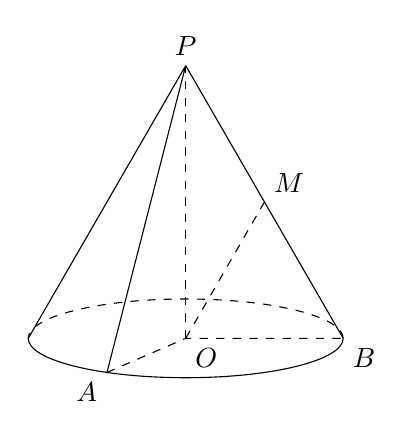
\begin{tikzpicture}[>=latex]
\draw (0,0) node [below right] {$O$} coordinate (O);
\draw (2,0) node [below right] {$B$} coordinate (B);
\draw (B) arc (0:-180:2 and 0.5);
\draw [dashed] (B) arc (0:180:2 and 0.5);
\draw [dashed] (O) --++ (0,{2*sqrt(3)}) node [above] {$P$} coordinate (P);
\draw ($(P)!0.5!(B)$) node [above right] {$M$} coordinate (M);
\draw ({2*cos(-120)},{0.5*sin(-120)}) node [below left] {$A$} coordinate (A);
\draw (P) -- (-2,0) (P) -- (A) (P) -- (B);
\draw [dashed] (A) -- (O) -- (B) (O) -- (M);
\end{tikzpicture}
\end{center}

\begin{center}
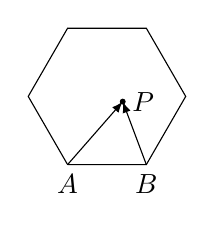
\begin{tikzpicture}[>=latex]
\draw (0,0) node [below] {$A$} coordinate (A) --++ (1,0) node [below] {$B$} coordinate (B) --++ (60:1) --++ (120:1) --++ (180:1) --++ (240:1) --++ (300:1);
\filldraw (0.7,0.8) circle (0.03) node [right] {$P$} coordinate (P);
\draw [->] (A) -- (P);
\draw [->] (B) -- (P);
\end{tikzpicture}
\end{center}

\begin{center}
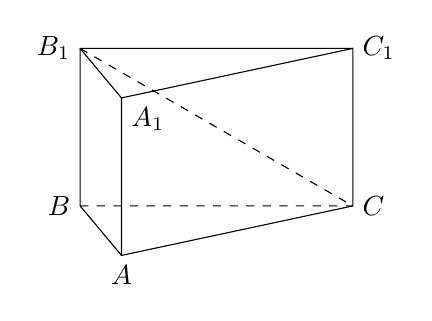
\begin{tikzpicture}[>=latex,scale = 2]
\draw (0,0,0) node [left] {$B$} coordinate (B);
\draw ({sqrt(3)},0,0) node [right] {$C$} coordinate (C);
\draw ($(B)!{1/3}!(C)$) ++ (0,0,{sqrt(2)/sqrt(3)}) node [below] {$A$} coordinate (A);
\draw (B) -- (A) -- (C) --++ (0,1) node [right] {$C_1$} coordinate (C1) --++ ({-sqrt(3)},0) node [left] {$B_1$} coordinate (B1) -- cycle;
\draw (A) --++ (0,1) node [below right] {$A_1$} coordinate (A1) -- (B1) (A1) -- (C1);
\draw [dashed] (B1) -- (C) (B) -- (C);
\end{tikzpicture}
\end{center}

\begin{center}
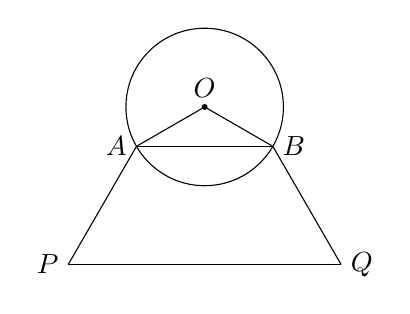
\begin{tikzpicture}[>=latex]
\draw (0,0) circle (1) node [above] {$O$} coordinate (O);
\filldraw (0,0) circle (0.03);
\draw (O) --++ (-30:1) node [right] {$B$} coordinate (B);
\draw (O) --++ (-150:1) node [left] {$A$} coordinate (A);
\draw (A) -- (B);
\draw (A) --++ (-120:{sqrt(3)}) node [left] {$P$} coordinate (P);
\draw (B) --++ (-60:{sqrt(3)}) node [right] {$Q$} coordinate (Q);
\draw (P) -- (Q);
\end{tikzpicture}
\end{center}

\begin{center}
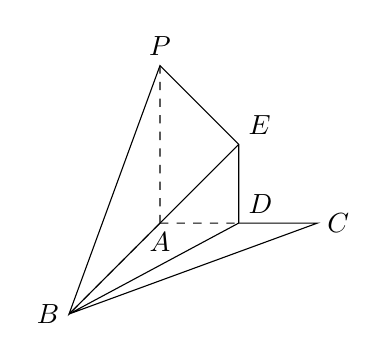
\begin{tikzpicture}[>=latex]
\draw (0,0,0) node [below] {$A$} coordinate (A);
\draw (1,0,0) node [above right] {$D$} coordinate (D);
\draw (2,0,0) node [right] {$C$} coordinate (C);
\draw (1,1,0) node [above right] {$E$} coordinate (E);
\draw (0,2,0) node [above] {$P$} coordinate (P);
\draw (0,0,3) node [left] {$B$} coordinate (B);
\draw (B) -- (D) -- (C) -- cycle;
\draw (D) -- (E) -- (P) -- (B) -- (E);
\draw [dashed] (A) -- (B) (A) -- (D) (A) -- (P);
\end{tikzpicture}
\end{center}

\begin{center}
\begin{tikzpicture}[>=latex]
\draw (0,0) -- (2,0) -- (2,1) -- (0,1) -- cycle;
\draw (0,1) -- (1,2) -- (2,1);
\draw (-0.1,0) -- (-0.5,0) (-0.1,1) -- (-0.5,1) (0.9,2) -- (-0.5,2);
\draw [->] (-0.3,0.2) -- (-0.3,0);
\draw [->] (-0.3,0.8) -- (-0.3,1);
\draw (-0.3,0.5) node {$1$};
\draw [->] (-0.3,1.2) -- (-0.3,1);
\draw [->] (-0.3,1.8) -- (-0.3,2);
\draw (-0.3,1.5) node {$1$};
\draw (0,-0.1) -- (0,-0.5) (2,-0.1) -- (2,-0.5);
\draw [->] (0.8,-0.3) -- (0,-0.3);
\draw [->] (1.2,-0.3) -- (2,-0.3);
\draw (1,-0.3) node {$2$};
\draw (1,-0.8) node {主视图};
\draw (3,0) -- (5,0) -- (5,1) -- (3,1) -- cycle;
\draw (3,1) -- (4,2) -- (5,1);
\draw (2.9,0) -- (2.5,0) (2.9,1) -- (2.5,1) (3.9,2) -- (2.5,2);
\draw [->] (2.7,0.2) -- (2.7,0);
\draw [->] (2.7,0.8) -- (2.7,1);
\draw (2.7,0.5) node {$1$};
\draw [->] (2.7,1.2) -- (2.7,1);
\draw [->] (2.7,1.8) -- (2.7,2);
\draw (2.7,1.5) node {$1$};
\draw (3,-0.1) -- (3,-0.5) (5,-0.1) -- (5,-0.5);
\draw [->] (3.8,-0.3) -- (3,-0.3);
\draw [->] (4.2,-0.3) -- (5,-0.3);
\draw (4,-0.3) node {$2$};
\draw (4,-0.8) node {左视图};
\draw (1,-2.5) circle (1);
\draw (0.9,-1.5) -- (-0.5,-1.5) (0.9,-3.5) -- (-0.5,-3.5);
\draw [->] (-0.3,-2.2) -- (-0.3,-1.5);
\draw [->] (-0.3,-2.8) -- (-0.3,-3.5);
\draw (-0.3,-2.5) node {$2$};
\draw (0,-2.6) -- (0,-4) (2,-2.6) -- (2,-4);
\draw [->] (0.8,-3.8) -- (0,-3.8);
\draw [->] (1.2,-3.8) -- (2,-3.8);
\draw (1,-3.8) node {$2$};
\draw (1,-4.2) node {俯视图};
\filldraw (1,-2.5) circle (0.03);
\end{tikzpicture}
\end{center}

\begin{center}
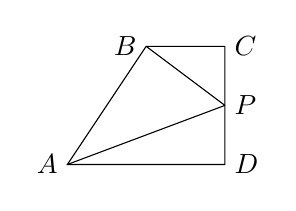
\begin{tikzpicture}[>=latex]
\draw (0,0) node [left] {$A$} coordinate (A) --++ (2,0) node [right] {$D$} coordinate (D) --++ (0,1.5) node [right] {$C$} coordinate (C) --++ (-1,0) node [left] {$B$} coordinate (B) -- cycle;
\draw (A) -- ($(C)!0.5!(D)$) node [right] {$P$} coordinate (P) (P) -- (B);
\end{tikzpicture}
\end{center}

\begin{center}
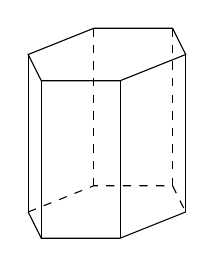
\begin{tikzpicture}[>=latex]
\draw (0,0,0) coordinate (A) --++ (1,0,0) coordinate (B) --++ ({1/2},0,{sqrt(3)/2}) coordinate (C) --++ ({-1/2},0,{sqrt(3)/2}) coordinate (D) --++ (-1,0,0) coordinate (E) --++ ({-1/2},0,{-sqrt(3)/2}) coordinate (F) -- cycle;
\draw [dashed] (A) --++ (0,-2,0) coordinate (A1);
\draw [dashed] (B) --++ (0,-2,0) coordinate (B1);
\draw (C) --++ (0,-2,0) coordinate (C1);
\draw (D) --++ (0,-2,0) coordinate (D1);
\draw (E) --++ (0,-2,0) coordinate (E1);
\draw (F) --++ (0,-2,0) coordinate (F1);
\draw (F1) -- (E1) -- (D1) -- (C1);
\draw [dashed] (F1) -- (A1) -- (B1) -- (C1);
\end{tikzpicture}
\end{center}

\begin{center}
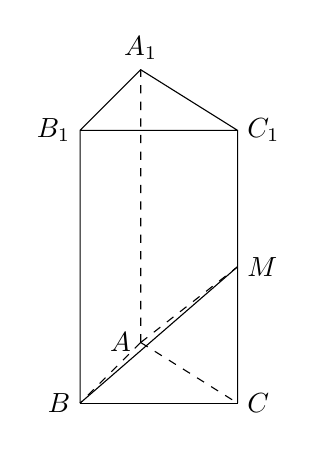
\begin{tikzpicture}[>=latex]
\draw (0,0,0) node [left] {$B$} coordinate (B) -- (2,0,0) node [right] {$C$} coordinate (C);
\draw (0,0,-2) node [left] {$A$} coordinate (A);
\draw (A) ++ (0,{2*sqrt(3)},0) node [above] {$A_1$} coordinate (A1);
\draw (B) ++ (0,{2*sqrt(3)},0) node [left] {$B_1$} coordinate (B1);
\draw (C) ++ (0,{2*sqrt(3)},0) node [right] {$C_1$} coordinate (C1);
\draw (B) -- (B1) -- (A1) -- (C1) -- (C) (B1) -- (C1);
\draw [dashed] (A) -- (A1) (A) -- (B) (A) -- (C);
\draw ($(C)!0.5!(C1)$) node [right] {$M$} coordinate (M);
\draw (M) -- (B);
\draw [dashed] (A) -- (M);
\end{tikzpicture}
\end{center}

\begin{center}
\begin{tikzpicture}[>=latex]
\filldraw (0,0) node [left] {$A$} coordinate (A) circle (0.03);
\filldraw (4,0) node [below] {$C$} coordinate (C) circle (0.03);
\filldraw (8,0) node [right] {$B$} coordinate (B) circle (0.03);
\draw (2,0) node [below] {$50$千米} (6,0) node [below] {$50$千米};
\filldraw (2.5,0) circle (0.03) node [above] {$P$};
\draw (A) -- (B);
\end{tikzpicture}
\end{center}

\begin{center}
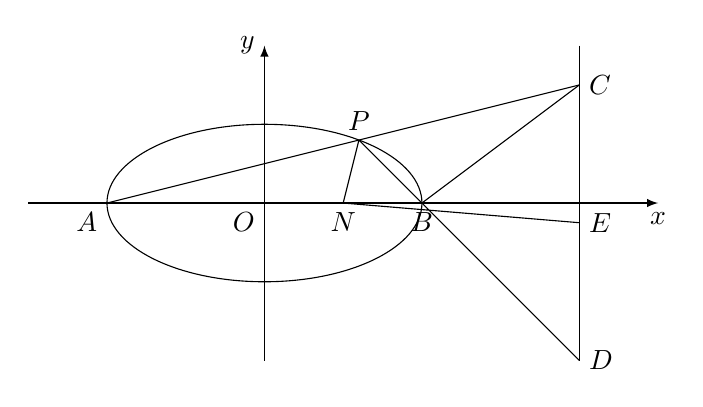
\begin{tikzpicture}[>=latex]
\draw [->] (-3,0) -- (5,0) node [below] {$x$};
\draw [->] (0,-2) -- (0,2) node [left] {$y$};
\draw (0,0) node [below left] {$O$};
\draw (4,2) -- (4,-2);
\draw (0,0) ellipse (2 and 1);
\draw (-2,0) node [below left] {$A$} coordinate (A) (2,0) node [below] {$B$} coordinate (B);
\draw (1.2,0.8) node [above] {$P$} coordinate (P);
\draw ($(A)!{6/3.2}!(P)$) node [right] {$C$} coordinate (C);
\draw ($(P)!{2.8/0.8}!(B)$) node [right] {$D$} coordinate (D);
\draw ($(C)!0.5!(D)$) node [right] {$E$} coordinate (E);
\draw (1,0) node [below] {$N$} coordinate (N);
\draw (P) -- (N) -- (E) (A) -- (C) (P) -- (D);
\draw (B) -- (C);
\end{tikzpicture}
\end{center}

\begin{center}
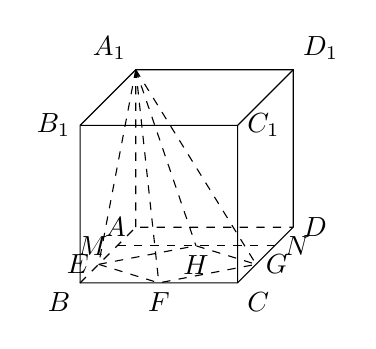
\begin{tikzpicture}[>=latex]
\draw (0,0) node [below left] {$B$} coordinate (B) --++ (2,0) node [below right] {$C$} coordinate (C) --++ (45:{2/2}) node [right] {$D$} coordinate (D)
--++ (0,2) node [above right] {$D_1$} coordinate (D1)
--++ (-2,0) node [above left] {$A_1$} coordinate (A1) --++ (225:{2/2}) node [left] {$B_1$} coordinate (B1) -- cycle;
\draw (B) ++ (2,2) node [right] {$C_1$} coordinate (C1) -- (C) (C1) --++ (45:{2/2}) (C1) --++ (-2,0);
\draw [dashed] (B) --++ (45:{2/2}) node [left] {$A$} coordinate (A) --++ (2,0) (A) --++ (0,2);
\draw [dashed] ($(A)!{1/3}!(B)$) node [left] {$M$} coordinate (M) -- ($(D)!{1/3}!(C)$) node [right] {$N$} coordinate (N);
\draw [dashed] ($(A)!{2/3}!(B)$) node [left] {$E$} coordinate (E) -- ($(B)!0.5!(C)$) node [below] {$F$} coordinate (F)--($(D)!{2/3}!(C)$) node [right] {$G$} coordinate (G);
\draw [dashed] (E) -- ($(M)!0.5!(N)$) node [below] {$H$} coordinate (H) -- (G);
\draw [dashed] (A1) -- (E) (A1) -- (F) (A1) -- (G) (A1) -- (H);
\end{tikzpicture}
\end{center}

\fourch{\begin{center}
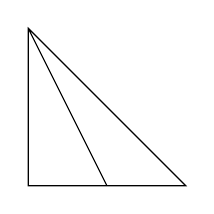
\begin{tikzpicture}[>=latex]
\draw (0,0) -- (2,0) -- (0,2) -- cycle (1,0) -- (0,2);
\end{tikzpicture}
\end{center}}{\begin{center}
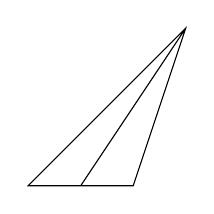
\begin{tikzpicture}[>=latex]
\draw (0,0) -- ({4/3},0) -- (2,2) -- cycle ({2/3},0) -- (2,2);
\end{tikzpicture}
\end{center}}{
\begin{center}
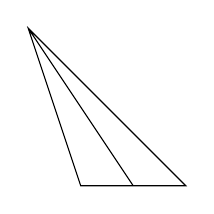
\begin{tikzpicture}[>=latex]
\draw ({2/3},0) -- (2,0) -- (0,2) -- cycle ({4/3},0) -- (0,2);
\end{tikzpicture}
\end{center}
}{\begin{center}
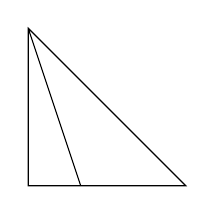
\begin{tikzpicture}[>=latex]
\draw (0,0) -- (2,0) -- (0,2) -- cycle ({2/3},0) -- (0,2);
\end{tikzpicture}
\end{center}
}

\begin{center}
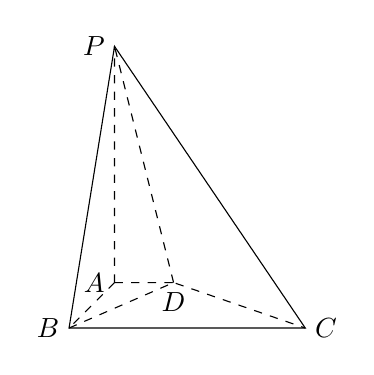
\begin{tikzpicture}[>=latex, scale = 0.75]
\draw (0,0,0) node [left] {$A$} coordinate (A);
\draw (0,4,0) node [left] {$P$} coordinate (P);
\draw (0,0,2) node [left] {$B$} coordinate (B);
\draw (1,0,0) node [below] {$D$} coordinate (D);
\draw (4,0,2) node [right] {$C$} coordinate (C);
\draw (B) -- (C) -- (P) -- cycle;
\draw [dashed] (A) -- (B) (A) -- (D) (A) -- (P) (B) -- (D) -- (C) (D) -- (P);
\end{tikzpicture}
\end{center}

\begin{center}
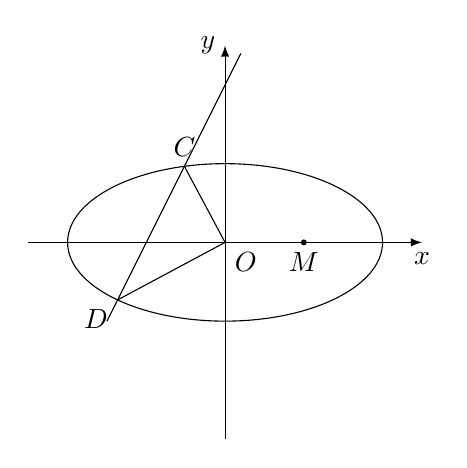
\begin{tikzpicture}[>=latex]
\draw [->] (-2.5,0) -- (2.5,0) node [below] {$x$};
\draw [->] (0,-2.5) -- (0,2.5) node [left] {$y$};
\draw (0,0) node [below right] {$O$};
\draw [name path = elli] (0,0) ellipse (2 and 1);
\draw [domain = -1.5:0.2, name path = line] plot (\x,{2*\x+2});
\draw [name intersections = {of = elli and line, by = {C,D}}];
\draw (0,0) -- (C) node [above] {$C$} (0,0) -- (D) node [below left] {$D$};
\filldraw (1,0) circle (0.03) node [below] {$M$};
\end{tikzpicture}
\end{center}

\begin{center}
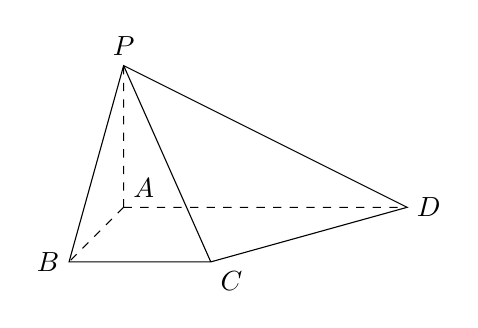
\begin{tikzpicture}[>=latex,scale = 1.8]
\draw (0,0,0) node [above right] {$A$} coordinate (A);
\draw (2,0,0) node [right] {$D$} coordinate (D);
\draw (0,0,1) node [left] {$B$} coordinate (B);
\draw (1,0,1) node [below right] {$C$} coordinate (C);
\draw (0,1,0) node [above] {$P$} coordinate (P);
\draw (P) -- (B) -- (C) -- (D) -- cycle (P) -- (C);
\draw [dashed] (A) -- (B) (A) -- (P) (A) -- (D);
\end{tikzpicture}
\end{center}

\begin{center}
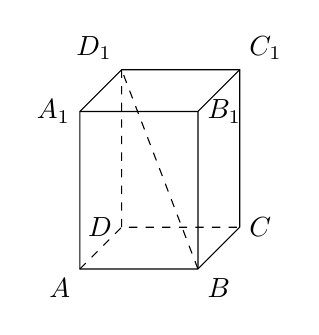
\begin{tikzpicture}[>=latex,scale = 0.5]
\draw (0,0) node [below left] {$A$} coordinate (A) --++ (3,0) node [below right] {$B$} coordinate (B) --++ (45:{3/2}) node [right] {$C$} coordinate (C)
--++ (0,4) node [above right] {$C_1$} coordinate (C1)
--++ (-3,0) node [above left] {$D_1$} coordinate (D1) --++ (225:{3/2}) node [left] {$A_1$} coordinate (A1) -- cycle;
\draw (A) ++ (3,4) node [right] {$B_1$} coordinate (B1) -- (B) (B1) --++ (45:{3/2}) (B1) --++ (-3,0);
\draw [dashed] (A) --++ (45:{3/2}) node [left] {$D$} coordinate (D) --++ (3,0) (D) --++ (0,4);
\draw [dashed] (B) -- (D1);
\end{tikzpicture}
\end{center}

\begin{center}
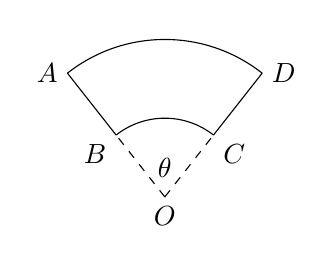
\begin{tikzpicture}[>=latex,scale = 0.2]
\def\t{10/15/pi*180}
\draw (0,0) node [below] {$O$} coordinate (O);
\draw [dashed] (0,0) --++ ({90-\t}:5) node [below right] {$C$} coordinate (C) (0,0) --++ ({90+\t}:5) node [below left] {$B$} coordinate (B);
\draw (B) -- ($(B)!-1!(O)$) node [left] {$A$} coordinate (A) (C) -- ($(C)!-1!(O)$) node [right] {$D$} coordinate (D);
\draw (D) arc ({90-\t}:{90+\t}:10) (C) arc ({90-\t}:{90+\t}:5);
\draw (O) pic ["$\theta$", angle eccentricity = 1.5, scale = 0.5] {angle = C--O--B};
\end{tikzpicture}
\end{center}

\begin{center}
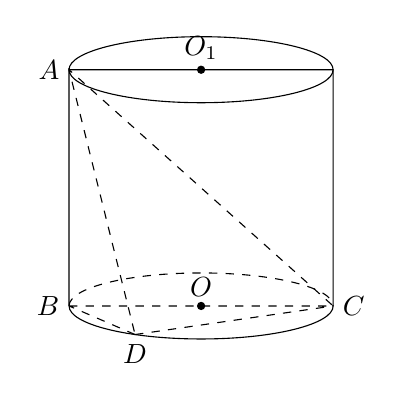
\begin{tikzpicture}[>=latex,scale = 1.5]
\draw ({-sqrt(5)/2},0) node [left] {$B$} coordinate (B) arc (180:360:{sqrt(5)/2} and {sqrt(5)/8}) node [right] {$C$} coordinate (C);
\draw [dashed] ({-sqrt(5)/2},0) arc (180:0:{sqrt(5)/2} and {sqrt(5)/8});
\draw (B) --++ (0,2) node [left] {$A$} coordinate (A) (C) --++ (0,2) -- (A);
\draw (A) arc (180:-180:{sqrt(5)/2} and {sqrt(5)/8});
\filldraw (0,0) circle (0.03) node [above] {$O$} coordinate (O);
\filldraw (O) ++ (0,2) circle (0.03) node [above] {$O_1$} coordinate (O1);
\draw ({sqrt(5)/2*cos(-120)},{sqrt(5)/8*sin(-120)}) node [below] {$D$} coordinate (D);
\draw [dashed] (D) -- (B) (D) -- (C) (B) -- (C) -- (A) -- (D);
\end{tikzpicture}
\end{center}

\begin{center}
\begin{tabular}{|c|c|c|c|c|c|}
\hline
$x$ & $1$ & $2$ & $3$ & $4$ & $5$ \\ \hline
$y$ & $2.2$ & $1$ & $2$ & $4.6$ & $7$ \\ \hline
\end{tabular}
\end{center}

\begin{center}
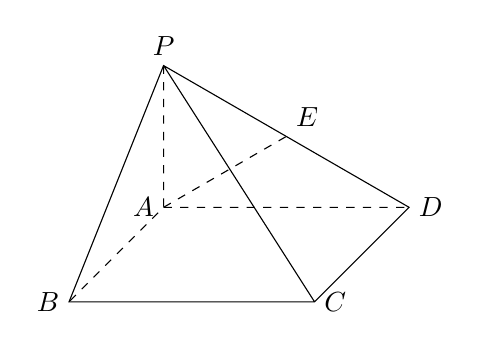
\begin{tikzpicture}[>=latex, scale = 1.8]
\draw (0,0,0) node [left] {$A$} coordinate (A);
\draw ({sqrt(3)},0,0) node [right] {$D$} coordinate (D);
\draw (0,0,{sqrt(3)}) node [left] {$B$} coordinate (B);
\draw ({sqrt(3)},0,{sqrt(3)}) node [right] {$C$} coordinate (C);
\draw (0,1,0) node [above] {$P$} coordinate (P);
\draw (P) -- (B) -- (C) -- (D) -- cycle (P) -- (C);
\draw [dashed] (P) -- (A) -- (B) (A) -- (D);
\draw ($(P)!0.5!(D)$) node [above right] {$E$} coordinate (E);
\draw [dashed] (A) -- (E);
\end{tikzpicture}
\end{center}

\begin{center}
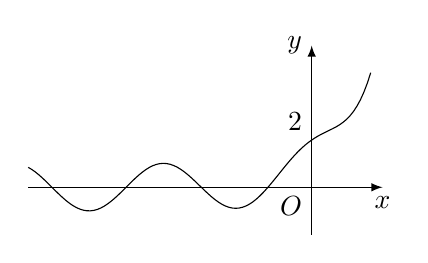
\begin{tikzpicture}[>=latex, scale = 0.3]
\draw [->] (-12,0) -- (3,0) node [below] {$x$};
\draw [->] (0,-2) -- (0,6) node [left] {$y$};
\draw (0,0) node [below left] {$O$};
\draw [domain = -12:2.5, samples = 100] plot (\x,{pow(2,\x)+cos(\x/pi*180)});
\draw (0,2) node [above left] {$2$};
\end{tikzpicture}
\end{center}

\begin{center}
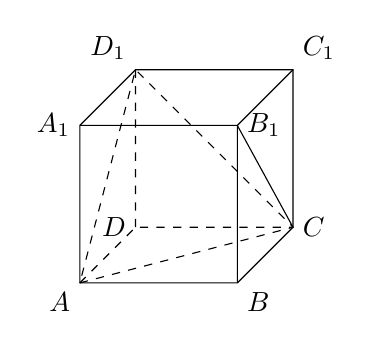
\begin{tikzpicture}[>=latex]
\draw (0,0) node [below left] {$A$} coordinate (A) --++ (2,0) node [below right] {$B$} coordinate (B) --++ (45:{2/2}) node [right] {$C$} coordinate (C)
--++ (0,2) node [above right] {$C_1$} coordinate (C1)
--++ (-2,0) node [above left] {$D_1$} coordinate (D1) --++ (225:{2/2}) node [left] {$A_1$} coordinate (A1) -- cycle;
\draw (A) ++ (2,2) node [right] {$B_1$} coordinate (B1) -- (B) (B1) --++ (45:{2/2}) (B1) --++ (-2,0);
\draw [dashed] (A) --++ (45:{2/2}) node [left] {$D$} coordinate (D) --++ (2,0) (D) --++ (0,2);
\draw (B1) -- (C);
\draw [dashed] (A) -- (C) -- (D1) -- cycle;
\end{tikzpicture}
\end{center}

\begin{center}
\begin{tikzpicture}[>=latex]
\draw (0,0,0) node [left] {$A$} coordinate (A);
\draw (1,0,0) node [right] {$B$} coordinate (B);
\draw (0,0,1) node [left] {$C$} coordinate (C);
\draw (A) ++ (0,2,0) node [above] {$A_1$} coordinate (A1);
\draw (B) ++ (0,2,0) node [right] {$B_1$} coordinate (B1);
\draw (C) ++ (0,2,0) node [left] {$C_1$} coordinate (C1);
\draw (A1) -- (B1) -- (B) -- (C) -- (C1) -- cycle (C1) -- (B1) (C1) -- (B);
\draw [dashed] (A) -- (C) (A) -- (B) (A) -- (A1) (A1) -- (B);
\draw (0.5,-0.8) node {图1};
\draw (A) ++ (3,0) node [left] {$A$} coordinate (A3);
\draw (B) ++ (3,0) node [right] {$B$} coordinate (B3);
\draw (C) ++ (3,0) node [left] {$C$} coordinate (C3);
\draw (C3) ++ (0,2) node [left] {$C_1$} coordinate (C4);
\draw (A3) ++ (0,2) node [above] {$A_1$} coordinate (A4);
\draw (B3) -- (C3) -- (C4) -- (A4) -- cycle (B3) -- (C4);
\draw [dashed] (A3) -- (B3) (A3) -- (C3) (A3) -- (A4);
\draw (B) ++ (4.5,0) node [right] {$B$} coordinate (B5);
\draw (B5) ++ (0,2) node [right] {$B_1$} coordinate (B6);
\draw (C1) ++ (4.5,0) node [left] {$C_1$} coordinate (C6);
\draw (A1) ++ (4.5,0) node [above] {$A_1$} coordinate (A6);
\draw (C6) -- (B5) -- (B6) -- (A6) -- cycle (B6) -- (C6);
\draw [dashed] (A6) -- (B5);
\draw (4.25,-0.8) node {图2};
\end{tikzpicture}
\end{center}

\begin{center}
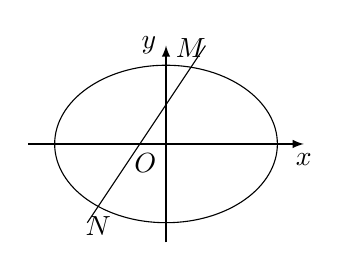
\begin{tikzpicture}[>=latex, scale = 0.5]
\draw [->] (-3.5,0) -- (3.5,0) node [below] {$x$};
\draw [->] (0,-2.5) -- (0,2.5) node [left] {$y$};
\draw (0,0) node [below left] {$O$};
\draw [name path = elli] (0,0) ellipse ({sqrt(8)} and 2);
\draw [name path = line] (1,2.5) -- (-2,-2);
\draw [name intersections = {of = elli and line, by = {M,N}}];
\draw (M) node [above] {$M$};
\draw (N) node [below] {$N$};
\end{tikzpicture}
\end{center}

\begin{center}
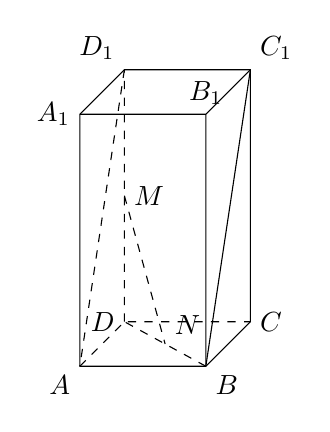
\begin{tikzpicture}[>=latex,scale = 0.8]
\draw (0,0) node [below left] {$A$} coordinate (A) --++ (2,0) node [below right] {$B$} coordinate (B) --++ (45:{2/2}) node [right] {$C$} coordinate (C)
--++ (0,4) node [above right] {$C_1$} coordinate (C1)
--++ (-2,0) node [above left] {$D_1$} coordinate (D1) --++ (225:{2/2}) node [left] {$A_1$} coordinate (A1) -- cycle;
\draw (A) ++ (2,4) node [above] {$B_1$} coordinate (B1) -- (B) (B1) --++ (45:{2/2}) (B1) --++ (-2,0);
\draw [dashed] (A) --++ (45:{2/2}) node [left] {$D$} coordinate (D) --++ (2,0) (D) --++ (0,4);
\draw ($(D)!0.5!(D1)$) node [right] {$M$} coordinate (M);
\draw ($(D)!0.5!(B)$) node [above right] {$N$} coordinate (N);
\draw [dashed] (B) -- (D) (M) -- (N) (D1) -- (A);
\draw (B) -- (C1);
\end{tikzpicture}
\end{center}

\begin{center}
\begin{tikzpicture}[>=latex]
\draw [->] (-2,0) -- (2,0) node [below] {$x$};
\draw [->] (0,-2) -- (0,2) node [left] {$y$};
\draw (0,0) node [below right] {$O$};
\filldraw (-1,0) circle (0.03) node [below] {$A$} coordinate (A);
\filldraw (1,0) circle (0.03) node [below] {$B$} coordinate (B);
\draw (-1.6,-1.6) -- (1.6,1.6) node [right] {$l$};
\draw (0.8,0.8) node [fill = white] {\rotatebox{45}{猫}};
\draw ({4/3},0.8) node {鼠};
\end{tikzpicture}
\end{center}

\begin{center}
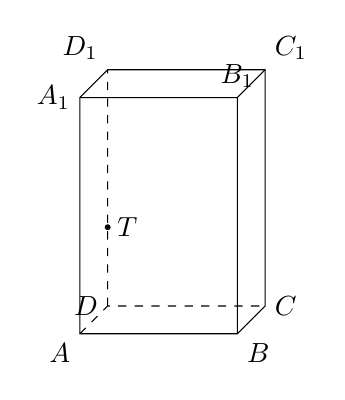
\begin{tikzpicture}[>=latex, scale = 0.5]
\draw (0,0) node [below left] {$A$} coordinate (A) --++ (4,0) node [below right] {$B$} coordinate (B) --++ (45:{2/2}) node [right] {$C$} coordinate (C)
--++ (0,6) node [above right] {$C_1$} coordinate (C1)
--++ (-4,0) node [above left] {$D_1$} coordinate (D1) --++ (225:{2/2}) node [left] {$A_1$} coordinate (A1) -- cycle;
\draw (A) ++ (4,6) node [above] {$B_1$} coordinate (B1) -- (B) (B1) --++ (45:{2/2}) (B1) --++ (-4,0);
\draw [dashed] (A) --++ (45:{2/2}) node [left] {$D$} coordinate (D) --++ (4,0) (D) --++ (0,6);
\filldraw ($(D)!{1/3}!(D1)$) circle (0.06) node [right] {$T$};
\end{tikzpicture}
\end{center}

\begin{center}
\begin{tikzpicture}[>=latex, scale = 0.4]
\draw (0,0) node [left] {$P_1$} coordinate (P1);
\draw ({sqrt(20)},0) node [right] {$P_2$} coordinate (P2);
\draw (P1) ++ (0,{sqrt(29)}) node [left] {$P_4$} coordinate (P4);
\draw (P2) ++ (0,{sqrt(29)}) node [right] {$P_3$} coordinate (P3);
\draw (P1) -- (P2) -- (P3) -- (P4) -- cycle;
\path [name path = c1] (P1) circle (4);
\path [name path = c2] (P3) circle (5);
\path [name intersections = {of = c1 and c2, by = {O,T}}];
\draw (O) node [above left] {$O$} -- (P1) (O) -- (P3);
\draw [->] (O) -- (P2);
\draw [->] (O) -- (P4);
\end{tikzpicture}
\end{center}

\begin{center}
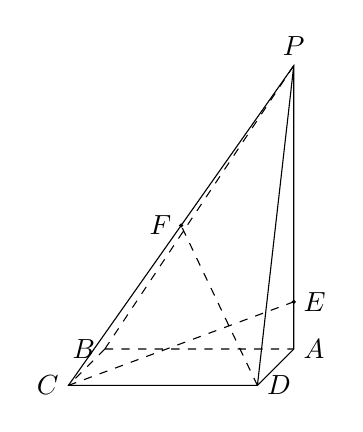
\begin{tikzpicture}[>=latex,scale = 0.6]
\draw (0,0,0) node [right] {$A$} coordinate (A);
\draw (0,6,0) node [above] {$P$} coordinate (P);
\draw (-4,0,0) node [left] {$B$} coordinate (B);
\draw (-4,0,2) node [left] {$C$} coordinate (C);
\draw (0,0,2) node [right] {$D$} coordinate (D);
\filldraw ($(C)!0.5!(P)$) circle (0.03) node [left] {$F$} coordinate (F);
\filldraw ($(A)!{1/6}!(P)$) circle (0.03) node [right] {$E$} coordinate (E);
\draw (A) -- (P) -- (C) -- (D) -- cycle (P) -- (D);
\draw [dashed] (B) -- (P) (B) -- (C) (B) -- (A) (C) -- (E) (D) -- (F);
\end{tikzpicture}
\end{center}

\begin{center}
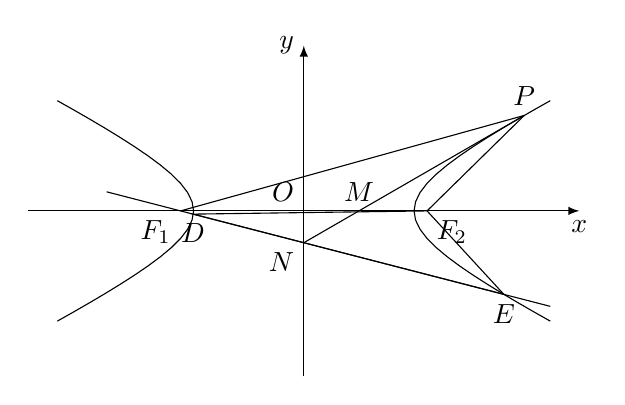
\begin{tikzpicture}[>=latex, scale = 0.7]
\draw [->] (-5,0) -- (5,0) node [below] {$x$};
\draw [->] (0,-3) -- (0,3) node [left] {$y$};
\draw (0,0) node [above left] {$O$};
\draw ({-sqrt(5)},0) node [below left] {$F_1$} coordinate (F1);
\draw ({sqrt(5)},0) node [below right] {$F_2$} coordinate (F2);
\draw (4,{sqrt(3)}) node [above] {$P$} coordinate (P);
\draw (P) -- (F1) (P) -- (F2);
\draw (1,0) node [above] {$M$} coordinate (M);
\draw ($(P)!{4/3}!(M)$) node [below left] {$N$} coordinate (N);
\draw (P) -- (N);
\draw [name path = line] ($(F1)!-0.6!(N)$) -- ($(F1)!3!(N)$);
\draw [name path = leftcurve, domain = -2:2] plot ({-sqrt(1+pow(\x,2))*2},\x);
\draw [name path = rightcurve, domain = -2:2] plot ({sqrt(1+pow(\x,2))*2},\x);
\draw [name intersections = {of = line and leftcurve, by = D}];
\draw [name intersections = {of = line and rightcurve, by = E}];
\draw (D) node [below] {$D$} -- (E) node [below] {$E$} -- (F2) -- cycle;
\end{tikzpicture}
\end{center}

\begin{center}
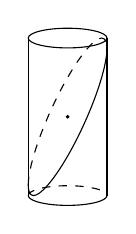
\begin{tikzpicture}[>=latex, scale = 0.5]
\draw (-1,-2) arc (180:360:1 and 0.25);
\draw (-1,2) arc (180:-180:1 and 0.25);
\draw [dashed] (-1,-2) arc (180:0:1 and 0.25);
\draw (-1,-2) -- (-1,2) (1,-2) -- (1,2);
\draw [domain = 180:360] plot ({cos(\x)},{-sqrt(3)+sin(\x)+sqrt(3)*(cos(\x)+1)});
\draw [domain = 180:0, dashed] plot ({cos(\x)},{-sqrt(3)+sin(\x)+sqrt(3)*(cos(\x)+1)});
\filldraw (0,0) circle (0.03);
\end{tikzpicture}
\end{center}

\begin{center}
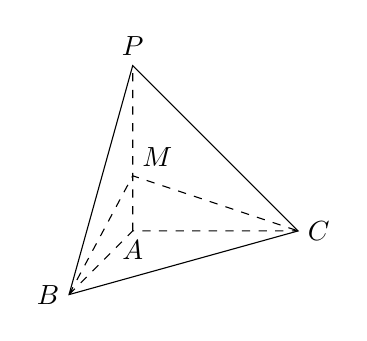
\begin{tikzpicture}[>=latex,scale = 0.7]
\draw (0,0,0) node [below] {$A$} coordinate (A);
\draw (3,0,0) node [right] {$C$} coordinate (C);
\draw (0,0,3) node [left] {$B$} coordinate (B);
\draw (0,3,0) node [above] {$P$} coordinate (P);
\draw (0,1,0) node [above right] {$M$} coordinate (M);
\draw (P) -- (B) -- (C) -- cycle;
\draw [dashed] (A) -- (P) (B) -- (A) -- (C) (B) -- (M) -- (C);
\end{tikzpicture}
\end{center}

\begin{center}
\begin{tikzpicture}[>=latex]
\filldraw (0,0) circle (0.05) node [left] {$A$} coordinate (A) -- (3,0) circle (0.05) node [right] {$B$} coordinate (B);
\path [name path = c1] (A) circle (3);
\path [name path = c2] (B) circle (1.8);
\path [name intersections = {of = c1 and c2, by = {P,Q}}];
\draw [dotted] (A) -- (P) node [above] {$P$} -- (B);
\filldraw (P) circle (0.03);
\draw [->] (3,1) -- (3,1.5) node [right] {北};
\draw (1.5,0) node [below] {居民生活区};
\end{tikzpicture}
\end{center}

\end{document}